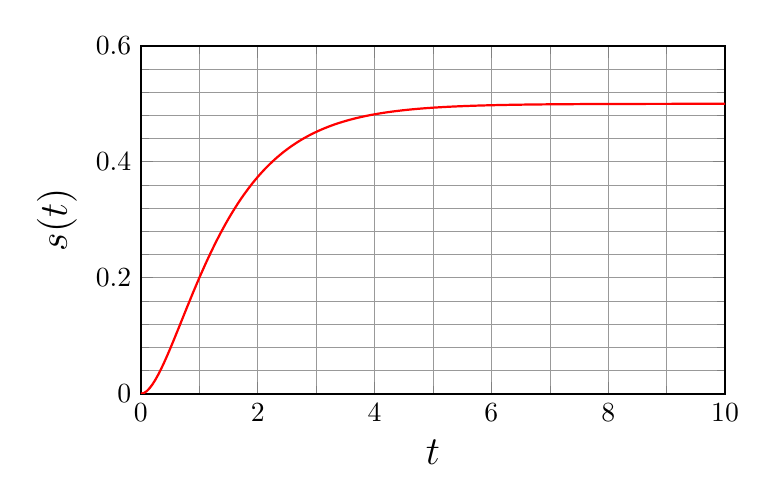
\begin{tikzpicture}
    \begin{axis}[
        width=9cm,
        height=6cm,
        legend style={draw=none},
        legend pos=south west,
        axis line style = thick,
        xmin=0,
        xmax=10,
        ymin=0,
        ymax=0.6,
        xlabel={$t$},
        ylabel={$s(t)$},
        label style={font=\Large},
        minor y tick num=4,
        minor x tick num=1,
        grid=both,
        grid style={line width=.2pt, draw=gray!80},
        major grid style={line width=.2pt,draw=gray!80},
    ]
        \addplot[thick,color=red,domain=0:10,samples=201]
        {0.5*(1-2*exp(-x)+exp(-2*x))};
    \end{axis}
\end{tikzpicture}

